\documentclass[a4paper,11pt]{article} %report
%oneside/twoside, openany/openright, twocolumn
\usepackage[T1]{fontenc} % codifica dei font
\usepackage[utf8]{inputenc} % lettere accentate da tastiera
\usepackage[italian]{babel} % lingua del documento
\usepackage{lipsum} % genera testo fittizio
\usepackage{url} % per scrivere gli indirizzi Internet
\usepackage{siunitx}
\usepackage{textcomp}
\usepackage{graphicx}
\usepackage{wrapfig}
\usepackage[colorlinks]{hyperref} %collegamenti ipertestuali --> \href{ h indirizzo Internet i }{ h testo del collegamento i }
\hypersetup{hidelinks}


\begin{document}

\author{Fuser Alessandro}
\title{FOG Detection and Prediction}
\maketitle

\tableofcontents

\newpage

\section{Future Learning for Detection and Prediction of Freezing of Gait in Parkinson's Disease\cite{uno}}
\subsection{Sommario}
In questo paper, vengono prima confrontati approcci di riconoscimento di feature basati sul dominio del tempo e feature statistiche con uno non supervisionato basato sull'analisi delle componenti principali, con il secondo che migliora il Freezing Index. Poi si analizza il problema della predizione del Freezing Of Gait (FoG), identificando dei pattern che avvengono prima degli episodi di FoG basandosi solo su dati provenienti da sensori di movimento. Si verrà a scoprire che le performance della predizione del FoG è altamente paziente dipendente.
\subsection{Articolo}
Ci sono alcune proprietà specifiche che differenziano i dati durante gli episodi di FoG rispetto alla normale camminata (es. l'energia del segnale della camminata è più spesso sulla banda 3-8Hz) ed, inoltre, si ha un caratteristico cambiamento nel modo di camminare prima di un episodio di FoG. Ma solo grazie a questi non possiamo essere certi di prevedere un episodio, anche perchè il deterioramento della normale camminata può essere espressa in vari modi e varia da paziente a paziente.\linebreak
Formuliamo dunque il problema della \textbf{Identificazione del FoG} come un problema di calssificazione a due classi: FoG contro normale camminata. Il problema della \textbf{Previsione del FoG}, invece, lo classifichiamo come un problema a tre classi, aggiungendo alle due precedenti una classe chiamata pre-FoG, dove faremo riconoscimento di tutte quelle caratteristiche specifiche che contraddistinguono il possibile presentarsi di un episodio di FoG. La durata di questo pre-FoG può essere variabile e può essere ricavato dallo studio dei segmenti di dati prima di un episodio di FoG (quando viene riconosciuto). Gli approcci di estrazione delle feature sono i seguenti:
\begin{enumerate}
\item Feature basate sulla frequenza, quindi Freezing Index (FI) ed energia totale nella banda di frequenza 0.5-8Hz;
\item Feature nel dominio del tempo e statistiche;
\item Apprendimento delle feature non supervisionato, ossia estrazione delle informazioni dai dati grezzi, senza basarsi su specifici domini.
\end{enumerate}
Il \textbf{FI} è definito come il rapporto tra la potenza contenuta nella banda di frequenza di freezing (3-8Hz) e quella della normale camminata (0.5-3Hz), che comporta il solo uso della FFT (Fast Fourier Transform). Vari classificatori sono stati usati per il problema a due classi, come Alberi di Decisione, Alberi/Foreste Random, Naive Bayes, basati su regole o su threshold. Invece di usare esplicite conoscenze per selezionare specifiche features, si possono estrarre quelle più caratteristiche tramite l'analisi delle componenti principali.  Risultati su dataset di attività pubbliche di riconoscimento mostrano che l'apprendento di feature nel metodo non supervisionato è molto più discriminativo dello state dell'arte basato sui precedenti approcci proposti (basati su tempo o frequenza). Per cui si propone di usare questo metodo per l'identificazione e la previsione di episodi di FoG, poichè le proprietà dei segnali di FoG e pre-FoG sono dipendenti dal soggetto e difficili da modellare.\linebreak
Il processo generale del \textbf{processamento e classificazione dei segnali} è il seguente: i segnali sono campionati e divisi in finestra con sovrapposizione parziale; per ogni finestra, le features vengono estratte ed i vettori risultati sono classificati in accordo con un modello già "allenato". Per questo lavoro, la lunghezza della finestra è di 1s (64 campioni) con una sovrapposizione di 0.25s(16 campioni), il classificatore usato è un albero di decisione per il suo basso bisogno di computazione. Ci siamo focalizzati nella selezione delle feature appropriate per la identificanzione e predizione del FoG, quindi \textit{l'ottimizzazione dei parametri di classificazione è fuori dai nostri scopi}. Nella fase di training del nostro sistema, abbiamo usato una classificazione delle feature basato sulla Mutua Informazione (MI), per trovare quelle più determinanti nel dominio del tempo e della frequenza (N$_{F}$).\linebreak
Sono stati scelti tre gruppi di feature:
\begin{enumerate}
\item FI e la somma delle energie delle bande di frequenza;
\item Feature nel dominio del tempo e statistiche, negli assi degli accelerometri o sui sensori;
\item Per imparare la struttura implicita dei dati, ogni finestra di 64 campioni per i tre accelerometri è riarrangiata in un vettore di 192; nella fase di training, un'analisi dei componenti principali (PCA) è applicata sull'intera matrice di dati.
\end{enumerate}
Assumiamo che l'andatura non può entrare in fase di FoG direttamente dalla camminata, ma c'è un deterioramento della stessa che, eventualmente, porta al FoG, rappresentata da un periodo T$_{prefog}$, il cui valore ottimale dipende dal paziente. Per il problema di detenzione, rimuoviamo dati per un periodo di T$_{prefog}$ prima di ogni evento di FoG nel set di allenamento, che ci porta ad avere un modello di classificazione più preciso per la classi FoG e WALK.\linebreak
Anche se vengono usati tre diversi accelerometri (anca, ginocchio e fondo schiena), ci si focalizza nei dati provenienti dal sensore sull'anca, poichè gli altri sono molto simili. L'inizio di un evento di FoG viene definito come lo stopparsi nel ritmo dell'andatura, mentre la sua fine è quando questa ricomincia.\linebreak
Le feature più importanti basate su MI sono l'Accelerazione dell'Energia Media (AAE), gli Autovalori della Matrice di covarianza dell'accelerazione sui 3 assi (EVA), l'intervallo, la Varianza, la Radice del Valore Medio e la Deviazione Standard.
Le istanze della classe pre-FoG non sono sempre molto differenti dalle classi WALK o FoG, per cui posso avere confusione, quindi è importante definire bene il T$_{prefog}$. Inoltre, ci sono delle limitazioni in merito all'ssunzione della classe pre-FoG:
\begin{itemize}
\item La natura differente degli episodi di FoG, per cui alcuni episodi avvengono senza che ci sia un'andatura prima del FoG, per cui non esiste quel deterioramento che abbiamo assunto;
\item La durata del T$_{prefog}$, che varia da paziente a paziente e da episodio a episodio.
\end{itemize}
\subsection{Conclusioni}
In questo lavoro, sono state analizzate le prestazioni di tre differenti approcci di estrazione delle feature per identificare FoG. Features basate nel dominio del tempo e statistiche sono state confrontate con un approccio non supervisionato sull'analisi delle principali componenti, mentre il FI è stato usato come base di riferimento. L'ultimo approccio migliora il FI di 7.1-8.1\% in termini di identificazione del FoG. Poi abbiamo cercato di analizzare il problema della predizione del FoG usando una problema a tre classi, assumendo un periodo T$_{prefog}$ di pre-FoG ed abbiamo ottenuto un risultato che dipende altamente dal paziente, con risultati fino al 56\% della misura di FI.\linebreak
L'uso delle feature non supervisionate è promettente, poichè catturano inportanti variazioni nei dati, senza il bisogno di esperti che selezionino manualmente quelle più importanti. Al fine di migliorare i risultati, altri metodi più complessi non supervisionati per l'apprendimento di feature possono essere testati (PCA che usa kernel non lineari, deep learning) e la durata fissa del T$_{prefog}$ deve essere riconsiderata. 

\section{Wearable assistant for Parkinson's disease patients with the freezing of gait symptom\cite{due}}
\subsection{Sommario}
Viene usato un sistema wearable che automaticamente riconosce FoG analizzando le componenti in frequenza coinvolte nel movimento. Quando un FoG viene riconosciuto, l'assistente fornisce un segnale auditorio ritmato che stimola il ritorno al camminare del paziente. La sensitività è del 73.1\% e la specificità del 81.6\%.
Il RAS (Rhytmic Auditory Stimulation) è stato riconosciuto come particolarmente efficace nello sbloccare FoG. Il suono di un metronomo regolare applicato come RAS con una frequenza del 110\% rispetto alla normale frequenza di camminata del paziente risulta ottimale nel mantenere la velocità dell'andatura e nel ridurne la variabilità. Il dispositivo wearable che usiamo mira a fornire il RAS solo durante il FoG o per inpedirne l'accadimento, quindi include algoritmi per il riconoscimento del FoG online. Questo manda i dati acquisiti ad un computer tramite una connessione Bluetooth ad una rate di 64Hz per il processo dei dati online. Il freeze viene riconosciuto usando una soglia ed i valori del \textbf{FI} oltre questa soglia vengono riconosciuti come FoG.\linebreak
\subsection{Articolo}
\begin{wrapfloat}{figure}{l}{0pt}
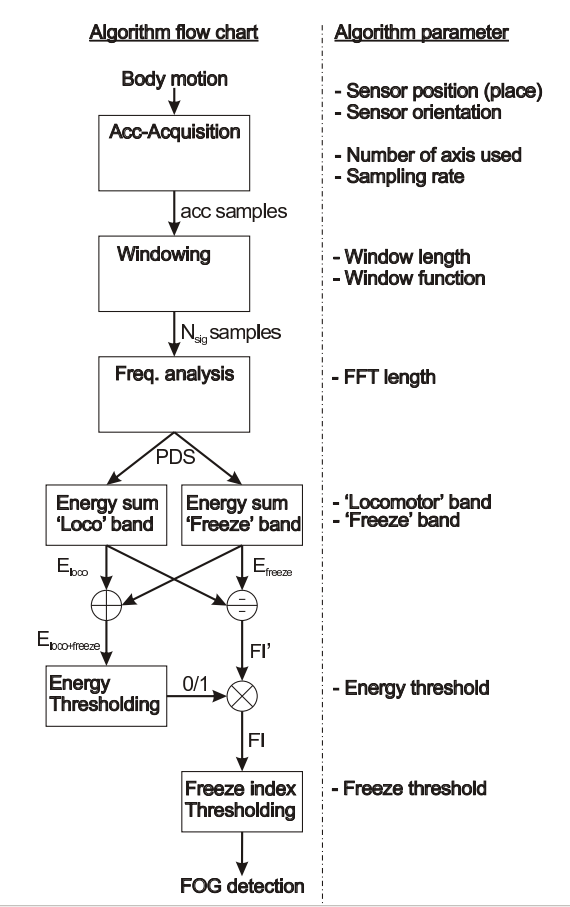
\includegraphics[scale=0.2]{Flow_chart_FOG.png}
\caption{Flow chart che descrive l'algoritmo di detenzione del FoG e tutti i suoi paramentri}
\end{wrapfloat}
Usando la \textbf{PSD} (Power Spectral Density), si riesce a definire un soglia di energia, chiamata \textit{PowerTH}, per distinguere lo stato dello "stare in piedi" dagli altri stati, poiché l'energia nello stare è sostanzialmente sempre minore rispetto al camminare o al FoG. Viene usato il \textit{Context Recognition Network} (CRN) Toolbox per l'implementazione dell'algoritmo nel dispositivo wearable, con una lunghezza di finestra di 4s, campionamento a 64Hz ed ogni finestratura è fatta a distanza di 0.5s. La durata del FoG varia da 0.5s a 40s, con il 50\% degli eventi che durano meno di 5.4s e il 93\% sotto i 20s. Il sistema doveva riconoscere il FoG entro 2s dal suo reale avvenimento per segnarlo come tale e le sensitività e specificità medie sono risultate, rispettivamente, del 73.1\% e del 81.6\%. Ma da paziente a paziente ci sono state grandi differenze, a causa dei differenti stili di camminata. Il sistema, quindi, dovrebbe essere regolato allo stile di camminata di ogni singolo paziente con un rapido set-up iniziale. Infatti, quando vengono ottimizzati i parametri in base allo stile di camminata, si riesce ad ottenere una sensitività dell'86.6\% e una specificità dell 92.4\%.\linebreak
Durante l'esperimento, anche i migliori risultati sono stati ottenuti dall'uso dell'asse verticale del sensore piazzato sul ginocchio, si è visto che non si perde molta accuratezza anche posizionando i sensori in altre parti del corpo. La latenza dell'algoritmo è dominato dalla lunghezza della finestra di campionamento, che si è dimostrata ottimale quando era settata su 4.5s.
\subsection{Conclusioni}
I calcoli complessi, come la FFT, che sono usati per il riconoscimento online del FoG, possono essere processati anche da device con poco consumo di potenza e della taglia di un bottone, quindi un dispositivo wearable va benissimo per lo scopo, indipendentemente dal suo posizionamento nel corpo. Il consiglio è quello di integrare l'algoritmo di detenzione direttamente nel dispositivo.



\pagebreak

\begin{thebibliography}{9}
\bibitem{uno} Sinziana Mazilu, Alberto Calatroni, Eran Gazit, Daniel Roggen, Jeffrey M.Hausdorff, Gerhard Troster,  
\emph{Future Learning for Detection and Prediction of Freezing of Gait in Parkinson's Disease}


\bibitem{due} Marc Bachlin, Meir Plotnik, Daniel Roggen, Inbal Maidan, Jeffrey M.Hausdorff, Nir Giladi, Gerhard Troster
\emph{Wearable assistant for Parkinson's disease patients with the freezing of gait symptom}, 2009
\end{thebibliography}

\end{document}